\subsection{Construction of semi-physical simulations}\label{sec:demo}
We wanted to test that a centralized communication system and artificial intelligence could improve traffic flow. In order to test the solution, we made a semi physical simulation where two cars approach an intersection simultaneously. We wanted to observe if the velocity of the vehicles were not drastically changed and, therefore, decreased the shockwave effect described in \secref{sec:traffic_congestion}.

We found a space at Accenture that was big enough to build the track. The power input on the Raspberry Pi vehicles is limited to a number between 40 and 100.  Since the server would adjust the vehicle's speed to avoid a collision, the intersection had to be at least 130cm away from the starting point. Otherwise, the server would adjust the vehicle's speed outside the equivalent power limits. Furthermore, the server prevented cars from driving before at least two vehicles have established a connection. Hence, both vehicles would start their journey simultaneously. We also placed the vehicles at the same distance from the intersection on their respective roads. Given these initial conditions, both vehicles were supposed to collide without the server's intervention. We also made the server log the velocity sent to the cars to track how much the cars' velocities changed.

Making the demo one hundred percent accurate was not possible in our circumstances due to the limitations of the Raspberry Pi. Furthermore, the vehicles were not able to receive the messages simultaneously. Consequently, this meant that they could start with a minor time difference. Another factor was that the trajectory of the vehicles was not always straight. However, even with these variances, the server was consistently able to navigate both cars through the intersection without collisions. \figref{fig:crashdemo} shows an example of a collision during a test demonstration.

\begin{figure}[h!]
	\centering
	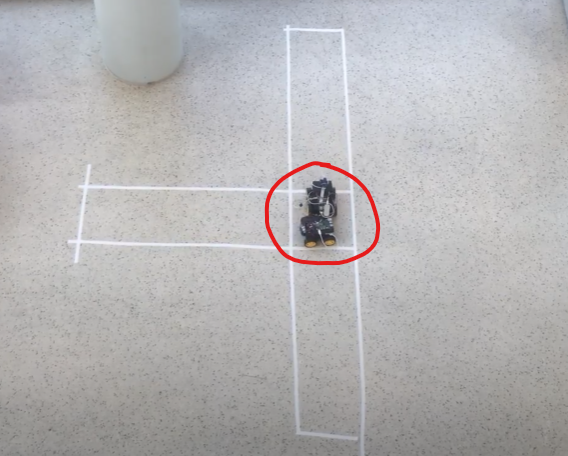
\includegraphics[width=0.9\linewidth]{figures/demo_crash}
	\caption{Here, we can observe the two cars colliding in the intersection. One of the cars started about 5 centimeters further behind the other car and started a few milliseconds later, resulting in a collision. Meanwhile, the server assumed they started simultaneously at the same distance from the intersection. In addition, the lengths of the vehicles were not accounted for.}
	\label{fig:crashdemo}
\end{figure}

Furthermore, the server did not account for the lengths of the vehicles during its calculations. Thus, we included the vehicles' length in the server's calculation. We also introduced a buffer zone to create a minimum gap between the cars. With these additions, we could consistently reproduce successful semi physical simulations.

When both vehicles had connected to the server, the cars would drive with an initial speed of 80 cm/s, the upper limit of the Raspberry Pi. Not long after they started to drive, the server recognized the cars approaching the intersection. Using the cars's velocity, position, and length, the server determined the target speed for one of the cars to avoid collision. After the other car had passed the intersection, the car that slowed down was told by the server to change its velocity back to 80 cm/s. \figref{fig:successdemo} is a snapshot of a successful test demo.

\begin{figure}[h!]
	\centering
	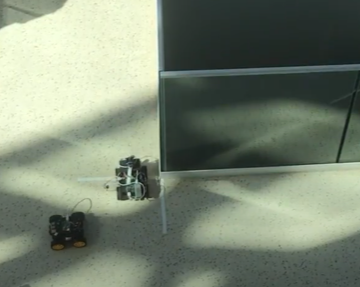
\includegraphics[width=0.9\linewidth]{figures/succsess_demo}
	\caption[Successful demo]{Here is an image of a successful simulation. The car to the left has just passed the intersection, marked as a square with white tape. The car furthest up is, therefore, about to adjust back to its original velocity. Here we can observe that the server prevents a collision.}
	\label{fig:successdemo}
\end{figure}